\documentclass[aps, twocolumn, superscriptaddress, floatfix, nofootinbib]{revtex4-2}

\usepackage[utf8]{inputenc}
\usepackage[T1]{fontenc}
\usepackage[brazilian]{babel}
\usepackage{amsmath, amssymb}
\usepackage{graphicx}
\usepackage{siunitx}
\usepackage{booktabs}
\usepackage{multirow}
\usepackage{hyperref}
\usepackage{float}

\sisetup{
  output-decimal-marker = {,},
  separate-uncertainty = true,
  multi-part-units = single,
  range-phrase = { a },
  list-separator = {; },
  list-final-separator = { e },
}

\begin{document}

\title{Experimento 6 --- Momento Magnético no Campo Magnético}

\author{Gabriel Simarelli Santos}
\author{Larissa Mello}

\affiliation{%
  Laboratório de Física Experimental~2 (NHT3028-15) --- Turma PREENCHER \\
  Prof.\ Breno Marques Gonçalves Teixeira \\
  Universidade Federal do ABC, Santo André, SP, Brasil
}

\date{\today}

\begin{abstract}
Neste experimento verificamos as relações de proporcionalidade previstas pela
teoria do torque magnético $\vec{\tau} = \vec{m}\times\vec{B}$ sobre uma espira
de corrente imersa no campo uniforme de bobinas de Helmholtz. Cinco
dependências funcionais foram medidas variando-se, uma de cada vez, a corrente
nas bobinas~($I'$), o número de espiras~($n$), o ângulo~($\alpha$), o
diâmetro~($d$) e a corrente na espira~($I$). Os dados foram ajustados pelo
método dos mínimos quadrados com minimização de~$\chi^2$ ponderado. Todas as
relações de proporcionalidade foram confirmadas com $R^2>0{,}97$, validando o
modelo $|\tau| = c\,n\,I\,(\pi d^2/4)\,I'\sin\alpha$. A constante geométrica
experimental das bobinas $c_{\text{exp}} = \SI{7,31(12)e-4}{\tesla\per\ampere}$
é compatível com o valor teórico $c_{\text{teo}} =
\SI{6,92e-4}{\tesla\per\ampere}$ dentro de $\sim 3\sigma$, confirmando a
consistência quantitativa do modelo.
\end{abstract}

\maketitle

%% ====================================================================
\section{Introdução e Objetivos}
%% ====================================================================

O momento de dipolo magnético é uma grandeza fundamental em eletromagnetismo,
responsável pela interação de espiras de corrente, ímãs permanentes e momentos
atômicos com campos magnéticos externos~\cite{Griffiths2017}. Quando um dipolo
magnético $\vec{m}$ é imerso em um campo magnético uniforme $\vec{B}$, surge um
torque $\vec{\tau}=\vec{m}\times\vec{B}$ que tende a alinhar o momento com o
campo. Esse princípio é explorado em motores elétricos, galvanômetros e em
técnicas de espectroscopia de ressonância magnética.

Para uma espira plana de $n$ voltas, área $A$ e corrente $I$, o módulo do
momento magnético vale $m = nIA$. Em campo uniforme produzido por bobinas de
Helmholtz, o torque assume a forma $|\tau| = m\,B\,\sin\alpha$, onde $\alpha$
é o ângulo entre $\vec{m}$ e $\vec{B}$. O objetivo deste experimento é
verificar experimentalmente cada uma das cinco dependências funcionais contidas
nessa expressão, variando-se: (1)~a intensidade do campo externo via corrente
$I'$ nas bobinas, (2)~o número de espiras $n$, (3)~o ângulo~$\alpha$, (4)~o
diâmetro $d$ da espira, e (5)~a corrente $I$ na espira.


%% ====================================================================
\section{Modelo Teórico}\label{sec:teoria}
%% ====================================================================

\subsection{Momento magnético e torque}

Para uma espira plana com $n$ voltas, diâmetro $d$ e percorrida por corrente
$I$, o momento de dipolo magnético é~\cite{Griffiths2017}
\begin{equation}\label{eq:momento}
  \vec{m} = n\,I\,\vec{A}\,, \qquad |\vec{A}| = \frac{\pi d^2}{4}\,,
\end{equation}
onde $\vec{A}$ é o vetor-área da espira. Imerso em campo magnético
$\vec{B}$, o torque resultante é
\begin{equation}\label{eq:torque}
  \vec{\tau} = \vec{m}\times\vec{B}\,,
\end{equation}
cujo módulo vale $|\tau| = m\,B\,\sin\alpha$, sendo $\alpha$ o ângulo entre
$\vec{m}$ e~$\vec{B}$.

\subsection{Campo das bobinas de Helmholtz}

Duas bobinas coaxiais idênticas, cada uma com $n_H$ espiras e raio $R_H$,
separadas por uma distância igual a $R_H$ (arranjo de Helmholtz), produzem um
campo aproximadamente uniforme na região central~\cite{PHYWE}:
\begin{equation}\label{eq:helmholtz}
  B = \left(\frac{4}{5}\right)^{3/2}\frac{\mu_0\,n_H}{R_H}\,I'
    \equiv c\,I'\,,
\end{equation}
onde $I'$ é a corrente nas bobinas e $c=(4/5)^{3/2}\mu_0 n_H/R_H$ é a
constante geométrica.

\subsection{Expressão geral do torque}

Substituindo~\eqref{eq:momento} e~\eqref{eq:helmholtz} em~\eqref{eq:torque}:
\begin{equation}\label{eq:geral}
  |\tau| = c\,n\,I\,\frac{\pi d^2}{4}\,I'\,\sin\alpha\,.
\end{equation}
Cada tarefa fixa quatro dos cinco parâmetros ($n$, $I$, $d$, $I'$, $\alpha$) e
varia o quinto, resultando em dependência linear na variável escolhida (ou em
$d^2$ para o diâmetro, ou em $\sin\alpha$ para o ângulo).

\subsection{Medida do torque}

O torque é medido indiretamente por um dinamômetro de torção que fornece a
força $F$ na extremidade de um braço de alavanca de comprimento $L$:
\begin{equation}\label{eq:tau_FL}
  \tau = F \times L\,.
\end{equation}


%% ====================================================================
\section{Descrição do Experimento}\label{sec:descricao}
%% ====================================================================

\subsection{Arranjo experimental}

A montagem segue o procedimento descrito na ref.~\cite{PHYWE} e no roteiro
experimental~\cite{Roteiro}. O campo magnético uniforme é gerado por um par de
bobinas de Helmholtz (PHYWE~06960.00; parâmetros nominais $n_H=154$ espiras,
$R_H=\SI{200}{\milli\metre}$), conectadas em série e alimentadas por uma fonte
de alimentação variável. No centro das bobinas, a espira de prova (conjunto
PHYWE~06404.00, com bobinas de 1, 2 e~3 espiras e diâmetros de
$\sim$\,60, 85 e~\SI{120}{\milli\metre}) é acoplada ao dinamômetro de torção
(PHYWE~02416.00). As correntes $I'$ (bobinas) e $I$ (espira) são medidas por
dois multímetros digitais de bancada Minipa MDM-8045A ($4\frac{1}{2}$
dígitos)~\cite{MDM8045A}.

\subsection{Especificações dos instrumentos}

\textit{Dinamômetro de torção:} faixa frontal~\SI{10}{\milli\newton},
subdivisão fina~\SI{0,1}{\milli\newton}, sensibilidade de
resposta~\SI{0,05}{\milli\newton}, braço de alavanca $L =
\SI{120}{\milli\metre}$~\cite{PHYWE}.

\textit{Multímetro Minipa MDM-8045A:} para corrente DC na escala de
\SI{20}{\ampere}, precisão $\pm(\SI{0,8}{\percent}\text{ da leitura} +
10\text{ dígitos}\times\SI{1}{\milli\ampere})$~\cite{MDM8045A}. Na escala de
\SI{2}{\ampere}: $\pm(\SI{0,8}{\percent} + 10\text{
díg.}\times\SI{100}{\micro\ampere})$.

\subsection{Procedimento}

Cinco séries de medidas foram realizadas, cada uma variando um único parâmetro
e mantendo os demais fixos, conforme o roteiro experimental~\cite{Roteiro}:

\textit{Tarefa~1} --- Torque $\tau$ em função da corrente $I'$ nas bobinas de
Helmholtz ($n=3$, $d=\SI{118,20}{\milli\metre}$, $I=\SI{3,004}{\ampere}$,
$\alpha=\ang{90}$).

\textit{Tarefa~2} --- Torque em função do número de espiras~$n$ ($I'=
\SI{3,016}{\ampere}$, $I=\SI{3,004}{\ampere}$, $d\approx
\SI{119}{\milli\metre}$, $\alpha=\ang{90}$).

\textit{Tarefa~3} --- Torque em função do ângulo~$\alpha$ ($n=3$, $d=
\SI{118,20}{\milli\metre}$, $I'=\SI{3,012}{\ampere}$,
$I=\SI{3,010}{\ampere}$).

\textit{Tarefa~4} --- Torque em função do diâmetro~$d$ ($n=1$,
$I'=\SI{3,032}{\ampere}$, $I=\SI{3,015}{\ampere}$, $\alpha=\ang{90}$).

\textit{Tarefa~5} --- Torque em função da corrente $I$ na espira ($n=3$, $d=
\SI{118,20}{\milli\metre}$, $I'=\SI{3,035}{\ampere}$, $\alpha=\ang{90}$).

Em todos os casos, a força $F$ (em \si{\milli\newton}) foi lida no dinamômetro
e o torque calculado por $\tau = F\times L$, com $L=\SI{120}{\milli\metre}$.


%% ====================================================================
\section{Resultados e Análise}\label{sec:resultados}
%% ====================================================================

\subsection{Estimativa de incertezas}\label{sec:incertezas}

\subsubsection{Incerteza na corrente}

A incerteza da corrente medida pelo multímetro MDM-8045A na escala de
\SI{20}{\ampere}~DC é~\cite{MDM8045A}
\begin{equation}\label{eq:sigI}
  \sigma_{I} = \SI{0,8}{\percent}\times|I| + 10\times\SI{1}{\milli\ampere}\,.
\end{equation}
Por exemplo, para $I'=\SI{3,019}{\ampere}$: $\sigma_{I'}=
0{,}008\times 3{,}019 + 0{,}010 = \SI{0,034}{\ampere}$.

\subsubsection{Incerteza no torque}

O torque é calculado a partir da força lida no dinamômetro:
$\tau = F\times L$. A propagação de incertezas fornece
\begin{equation}\label{eq:sigtau}
  \sigma_\tau = \sqrt{(L\,\sigma_F)^2 + (F\,\sigma_L)^2}\,,
\end{equation}
onde $\sigma_F = \SI{0,05}{\milli\newton}$ (sensibilidade do dinamômetro) e
$\sigma_L = \SI{1}{\milli\metre}$ (incerteza mecânica do braço). Para o ponto
$F=\SI{1,92}{\milli\newton}$, obtém-se $\sigma_\tau = \SI{0,006}{\milli\newton
\cdot\metre}$, dominado pelo termo $L\,\sigma_F$.

\subsubsection{Transferência de incertezas e MMQ ponderado}

Para o ajuste linear $y=ax+b$ pelo método dos mínimos quadrados (MMQ), as
incertezas em~$x$ são transferidas para~$y$~\cite{Vuolo}:
\begin{equation}\label{eq:transf}
  \sigma_y^{\,2} = \sigma_{y_0}^{\,2}
    + \left(\frac{dy}{dx}\cdot\sigma_x\right)^2,
\end{equation}
onde $dy/dx$ é estimado pelo coeficiente angular de uma regressão linear
simples preliminar. O ajuste final usa \texttt{numpy.polyfit} com pesos
$w_i=1/\sigma_{y,i}$ e extração da matriz de covariância~\cite{Vuolo}.

A qualidade é avaliada pelo $\chi^2$ reduzido
\begin{equation}\label{eq:chi2}
  \chi^2_{\text{red}}
    = \frac{1}{N-2}\sum_{i=1}^{N}
      \left(\frac{\hat{y}_i - y_i}{\sigma_{y,i}}\right)^2,
\end{equation}
pelo coeficiente de correlação $R^2$ e pelo gráfico de resíduos
$(\hat{y}_i - y_i)$ \emph{vs.}~$x_i$. Um bom ajuste apresenta
$\chi^2_{\text{red}}\approx 1$, $R^2$ próximo de~1 e resíduos aleatoriamente
distribuídos em torno de zero~\cite{Vuolo}.


%% -------------------------------------------------------------------
\subsection{Tarefa 1: $\tau$ \emph{vs.} $I'$}
%% -------------------------------------------------------------------

Os dados são apresentados na Tabela~\ref{tab:t1}.

\begin{table}[H]
\caption{Tarefa~1: força e torque em função da corrente $I'$ nas bobinas de
Helmholtz. Condições fixas: $n=3$, $d=\SI{118,20}{\milli\metre}$,
$I=\SI{3,004}{\ampere}$, $\alpha=\ang{90}$.}\label{tab:t1}
\begin{ruledtabular}
\begin{tabular}{cccccc}
$I'$ (A) & $\sigma_{I'}$ (A) & $F$ (mN) & $\tau$ (mN$\cdot$m) & $\sigma_\tau$ & $\sigma_\tau^{\text{transf}}$ \\
\hline
0,372 & 0,013 & 0,33 & 0,0396 & 0,0060 & 0,0061 \\
0,607 & 0,015 & 0,44 & 0,0528 & 0,0060 & 0,0061 \\
0,909 & 0,017 & 0,61 & 0,0732 & 0,0060 & 0,0062 \\
1,204 & 0,020 & 0,83 & 0,0996 & 0,0061 & 0,0062 \\
1,501 & 0,022 & 1,01 & 0,1212 & 0,0061 & 0,0063 \\
1,802 & 0,024 & 1,19 & 0,1428 & 0,0061 & 0,0064 \\
2,102 & 0,027 & 1,37 & 0,1644 & 0,0062 & 0,0065 \\
2,410 & 0,029 & 1,51 & 0,1812 & 0,0062 & 0,0065 \\
2,716 & 0,032 & 1,72 & 0,2064 & 0,0062 & 0,0066 \\
3,019 & 0,034 & 1,92 & 0,2304 & 0,0063 & 0,0068 \\
\end{tabular}
\end{ruledtabular}
\end{table}

A relação esperada $\tau = a\,I' + b$ é linear, dispensando linearização. O
ajuste MMQ ponderado fornece:
\begin{align}
  a &= \SI{0,0723(9)}{\milli\newton\cdot\metre\per\ampere}\,,\nonumber\\
  b &= \SI{0,011(2)}{\milli\newton\cdot\metre}\,,\nonumber\\
  \chi^2_{\text{red}} &= 0{,}15\,,\quad R^2 = 0{,}9988\,.\label{eq:fit1}
\end{align}

O gráfico de $\tau$ \emph{vs.}~$I'$ com a reta de ajuste e o respectivo
gráfico de resíduos são mostrados na Fig.~\ref{fig:t1}.

\begin{figure}[H]
  \centering
  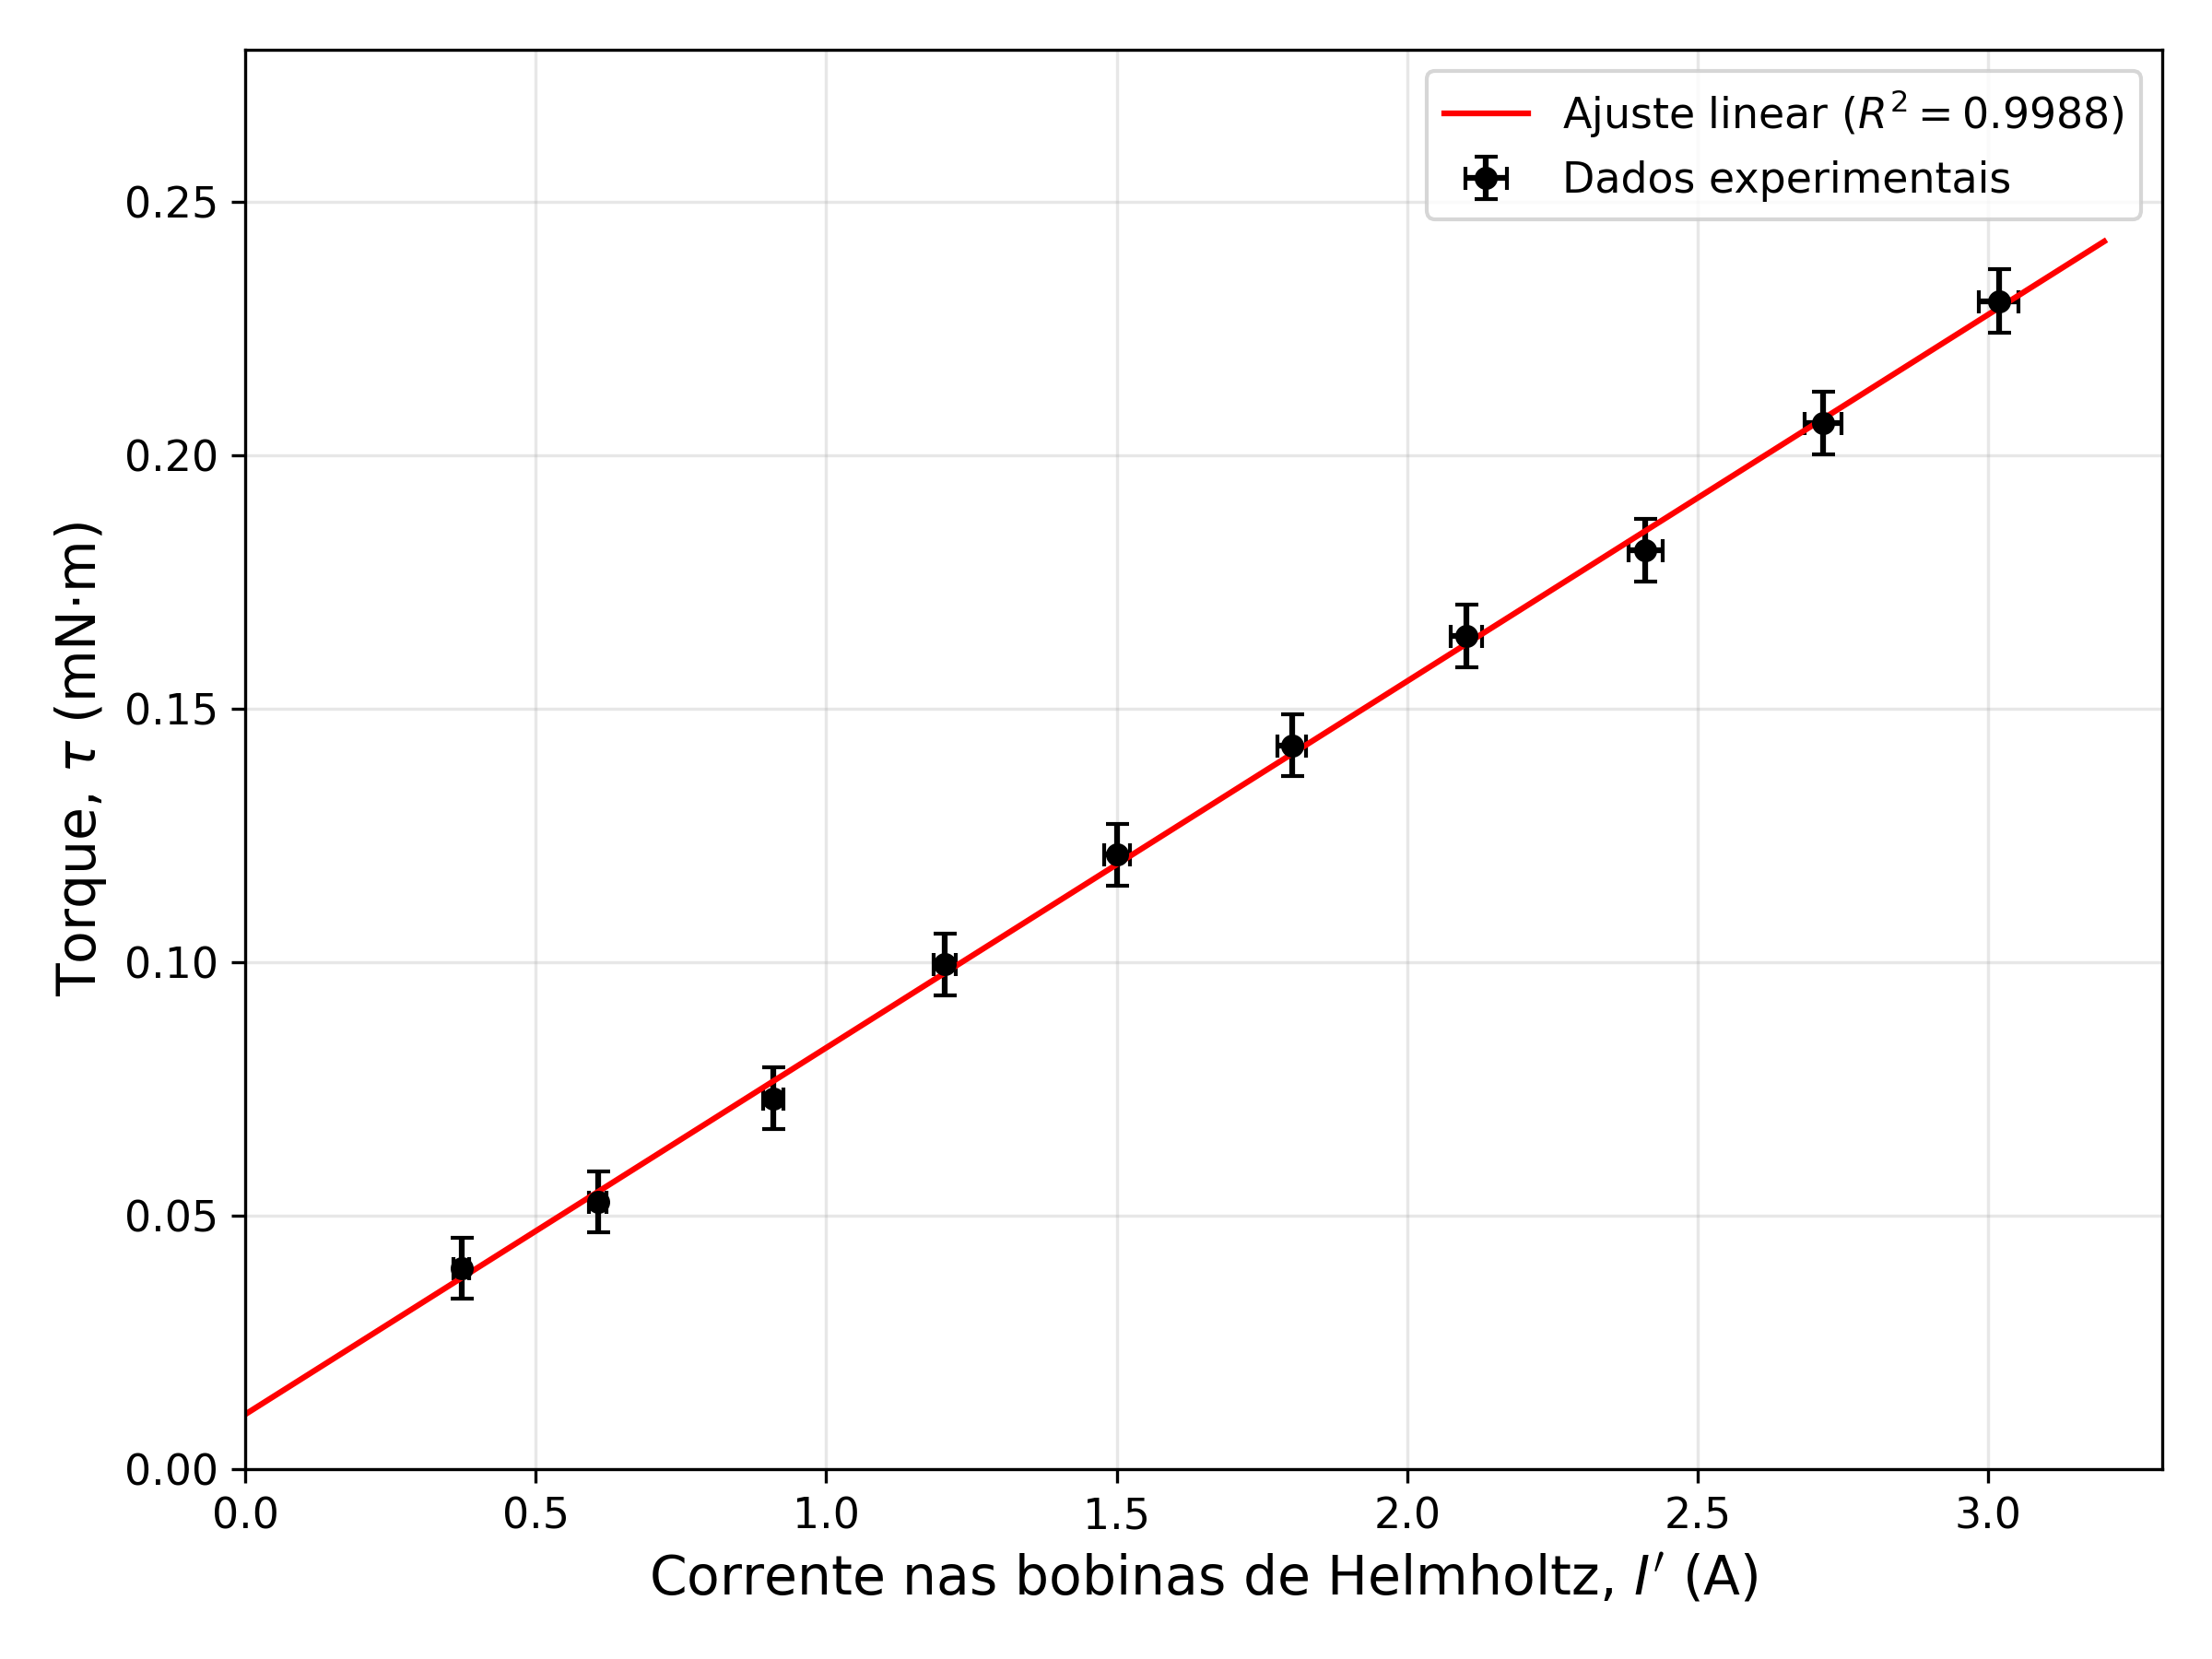
\includegraphics[width=\columnwidth]{tarefa1_tau_vs_Ip.png}
  \caption{Tarefa~1: torque $\tau$ em função da corrente nas bobinas $I'$.
  Pontos: dados experimentais com barras de erro. Reta: ajuste MMQ
  ponderado.}\label{fig:t1}
\end{figure}


%% -------------------------------------------------------------------
\subsection{Tarefa 2: $\tau$ \emph{vs.} $n$}
%% -------------------------------------------------------------------

Os resultados são apresentados na Tabela~\ref{tab:t2}. Como $n$ é uma variável
discreta sem incerteza, não há transferência de $\sigma_x$ para $\sigma_y$.

\begin{table}[H]
\caption{Tarefa~2: torque em função do número de espiras. Condições fixas:
$I'=\SI{3,016}{\ampere}$, $I=\SI{3,004}{\ampere}$,
$\alpha=\ang{90}$.}\label{tab:t2}
\begin{ruledtabular}
\begin{tabular}{cccc}
$n$ & $d$ (mm) & $F$ (mN) & $\tau$ (mN$\cdot$m) \\
\hline
1 & 119,70 & 0,65 & 0,078 \\
2 & 119,00 & 1,11 & 0,133 \\
3 & 118,20 & 1,92 & 0,230 \\
\end{tabular}
\end{ruledtabular}
\end{table}

O ajuste linear $\tau = a\,n + b$ resulta em
\begin{align}
  a &= \SI{0,076(12)}{\milli\newton\cdot\metre\per\text{espira}}\,,\nonumber\\
  b &= \SI{-0,005(26)}{\milli\newton\cdot\metre}\,,\nonumber\\
  \chi^2_{\text{red}} &= 7{,}8\,,\quad R^2 = 0{,}975\,.\label{eq:fit2}
\end{align}

O valor elevado de $\chi^2_{\text{red}}$ reflete a dispersão inerente a apenas
3~pontos (1~grau de liberdade). A Fig.~\ref{fig:t2} confirma a tendência
linear.

\begin{figure}[H]
  \centering
  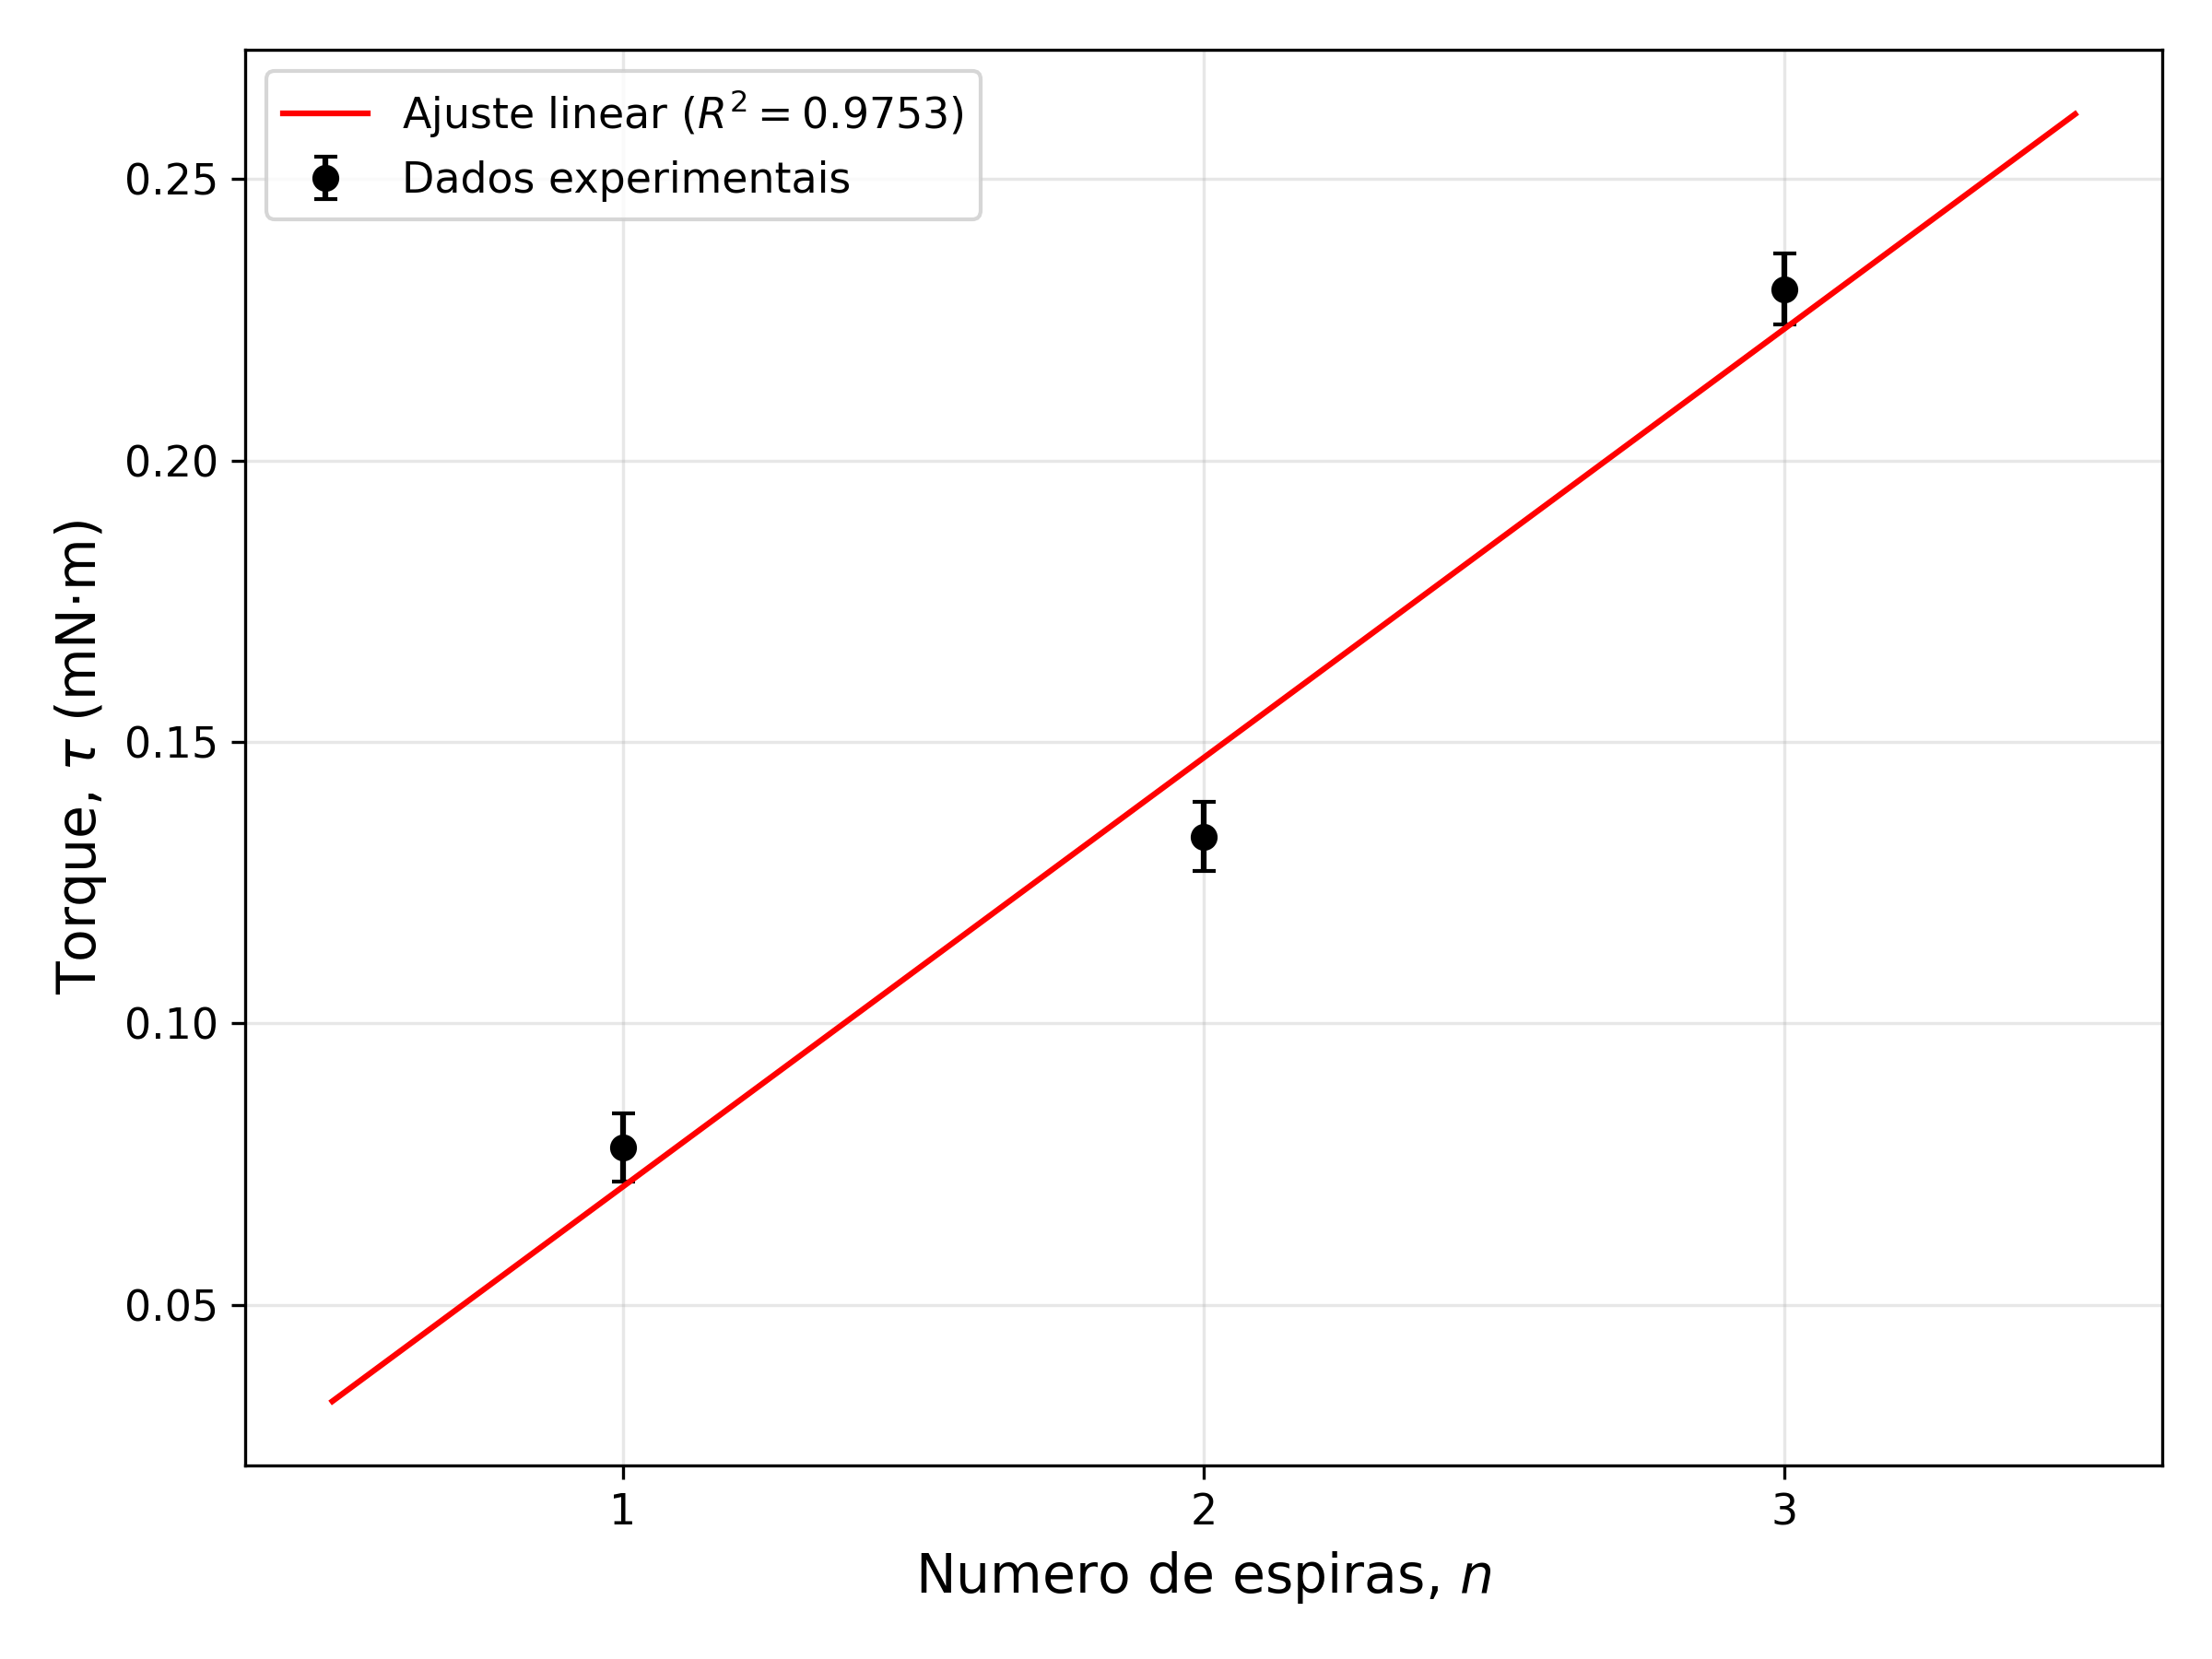
\includegraphics[width=\columnwidth]{tarefa2_tau_vs_n.png}
  \caption{Tarefa~2: $\tau$ em função de~$n$.}\label{fig:t2}
\end{figure}


%% -------------------------------------------------------------------
\subsection{Tarefa 3: $\tau$ \emph{vs.} $\sin\alpha$}
%% -------------------------------------------------------------------

A Tabela~\ref{tab:t3} apresenta os dados com a conversão para $\sin\alpha$.

\begin{table}[H]
\caption{Tarefa~3: torque em função do ângulo. Condições fixas: $n=3$, $d=
\SI{118,20}{\milli\metre}$, $I'=\SI{3,012}{\ampere}$,
$I=\SI{3,010}{\ampere}$.}\label{tab:t3}
\begin{ruledtabular}
\begin{tabular}{ccccc}
$\alpha$ ($^\circ$) & $\sin\alpha$ & $\sigma_{\sin\alpha}$ & $F$ (mN) & $\tau$ (mN$\cdot$m) \\
\hline
0  & 0,000 & 0,035 & 0,00 & 0,000 \\
15 & 0,259 & 0,034 & 0,38 & 0,046 \\
30 & 0,500 & 0,030 & 0,75 & 0,090 \\
45 & 0,707 & 0,025 & 1,12 & 0,134 \\
60 & 0,866 & 0,017 & 1,68 & 0,202 \\
75 & 0,966 & 0,009 & 1,71 & 0,205 \\
90 & 1,000 & 0,000 & 1,91 & 0,229 \\
\end{tabular}
\end{ruledtabular}
\end{table}

A incerteza em $\sin\alpha$ é propagada por
$\sigma_{\sin\alpha}=|\cos\alpha|\,\sigma_\alpha$, adotando-se
$\sigma_\alpha=\ang{2}$ (resolução dos entalhes do suporte). O ajuste
$\tau = a\sin\alpha + b$ fornece
\begin{align}
  a &= \SI{0,234(16)}{\milli\newton\cdot\metre}\,,\nonumber\\
  b &= \SI{-0,014(12)}{\milli\newton\cdot\metre}\,,\nonumber\\
  \chi^2_{\text{red}} &= 2{,}9\,,\quad R^2 = 0{,}979\,.\label{eq:fit3}
\end{align}

O valor de $\chi^2_{\text{red}}$ moderadamente acima de~1 pode indicar que a
incerteza angular está subestimada ou que houve efeito de histerese na medida
de $\alpha = \ang{60}$--\ang{75}. A Fig.~\ref{fig:t3} mostra o ajuste.

\begin{figure}[H]
  \centering
  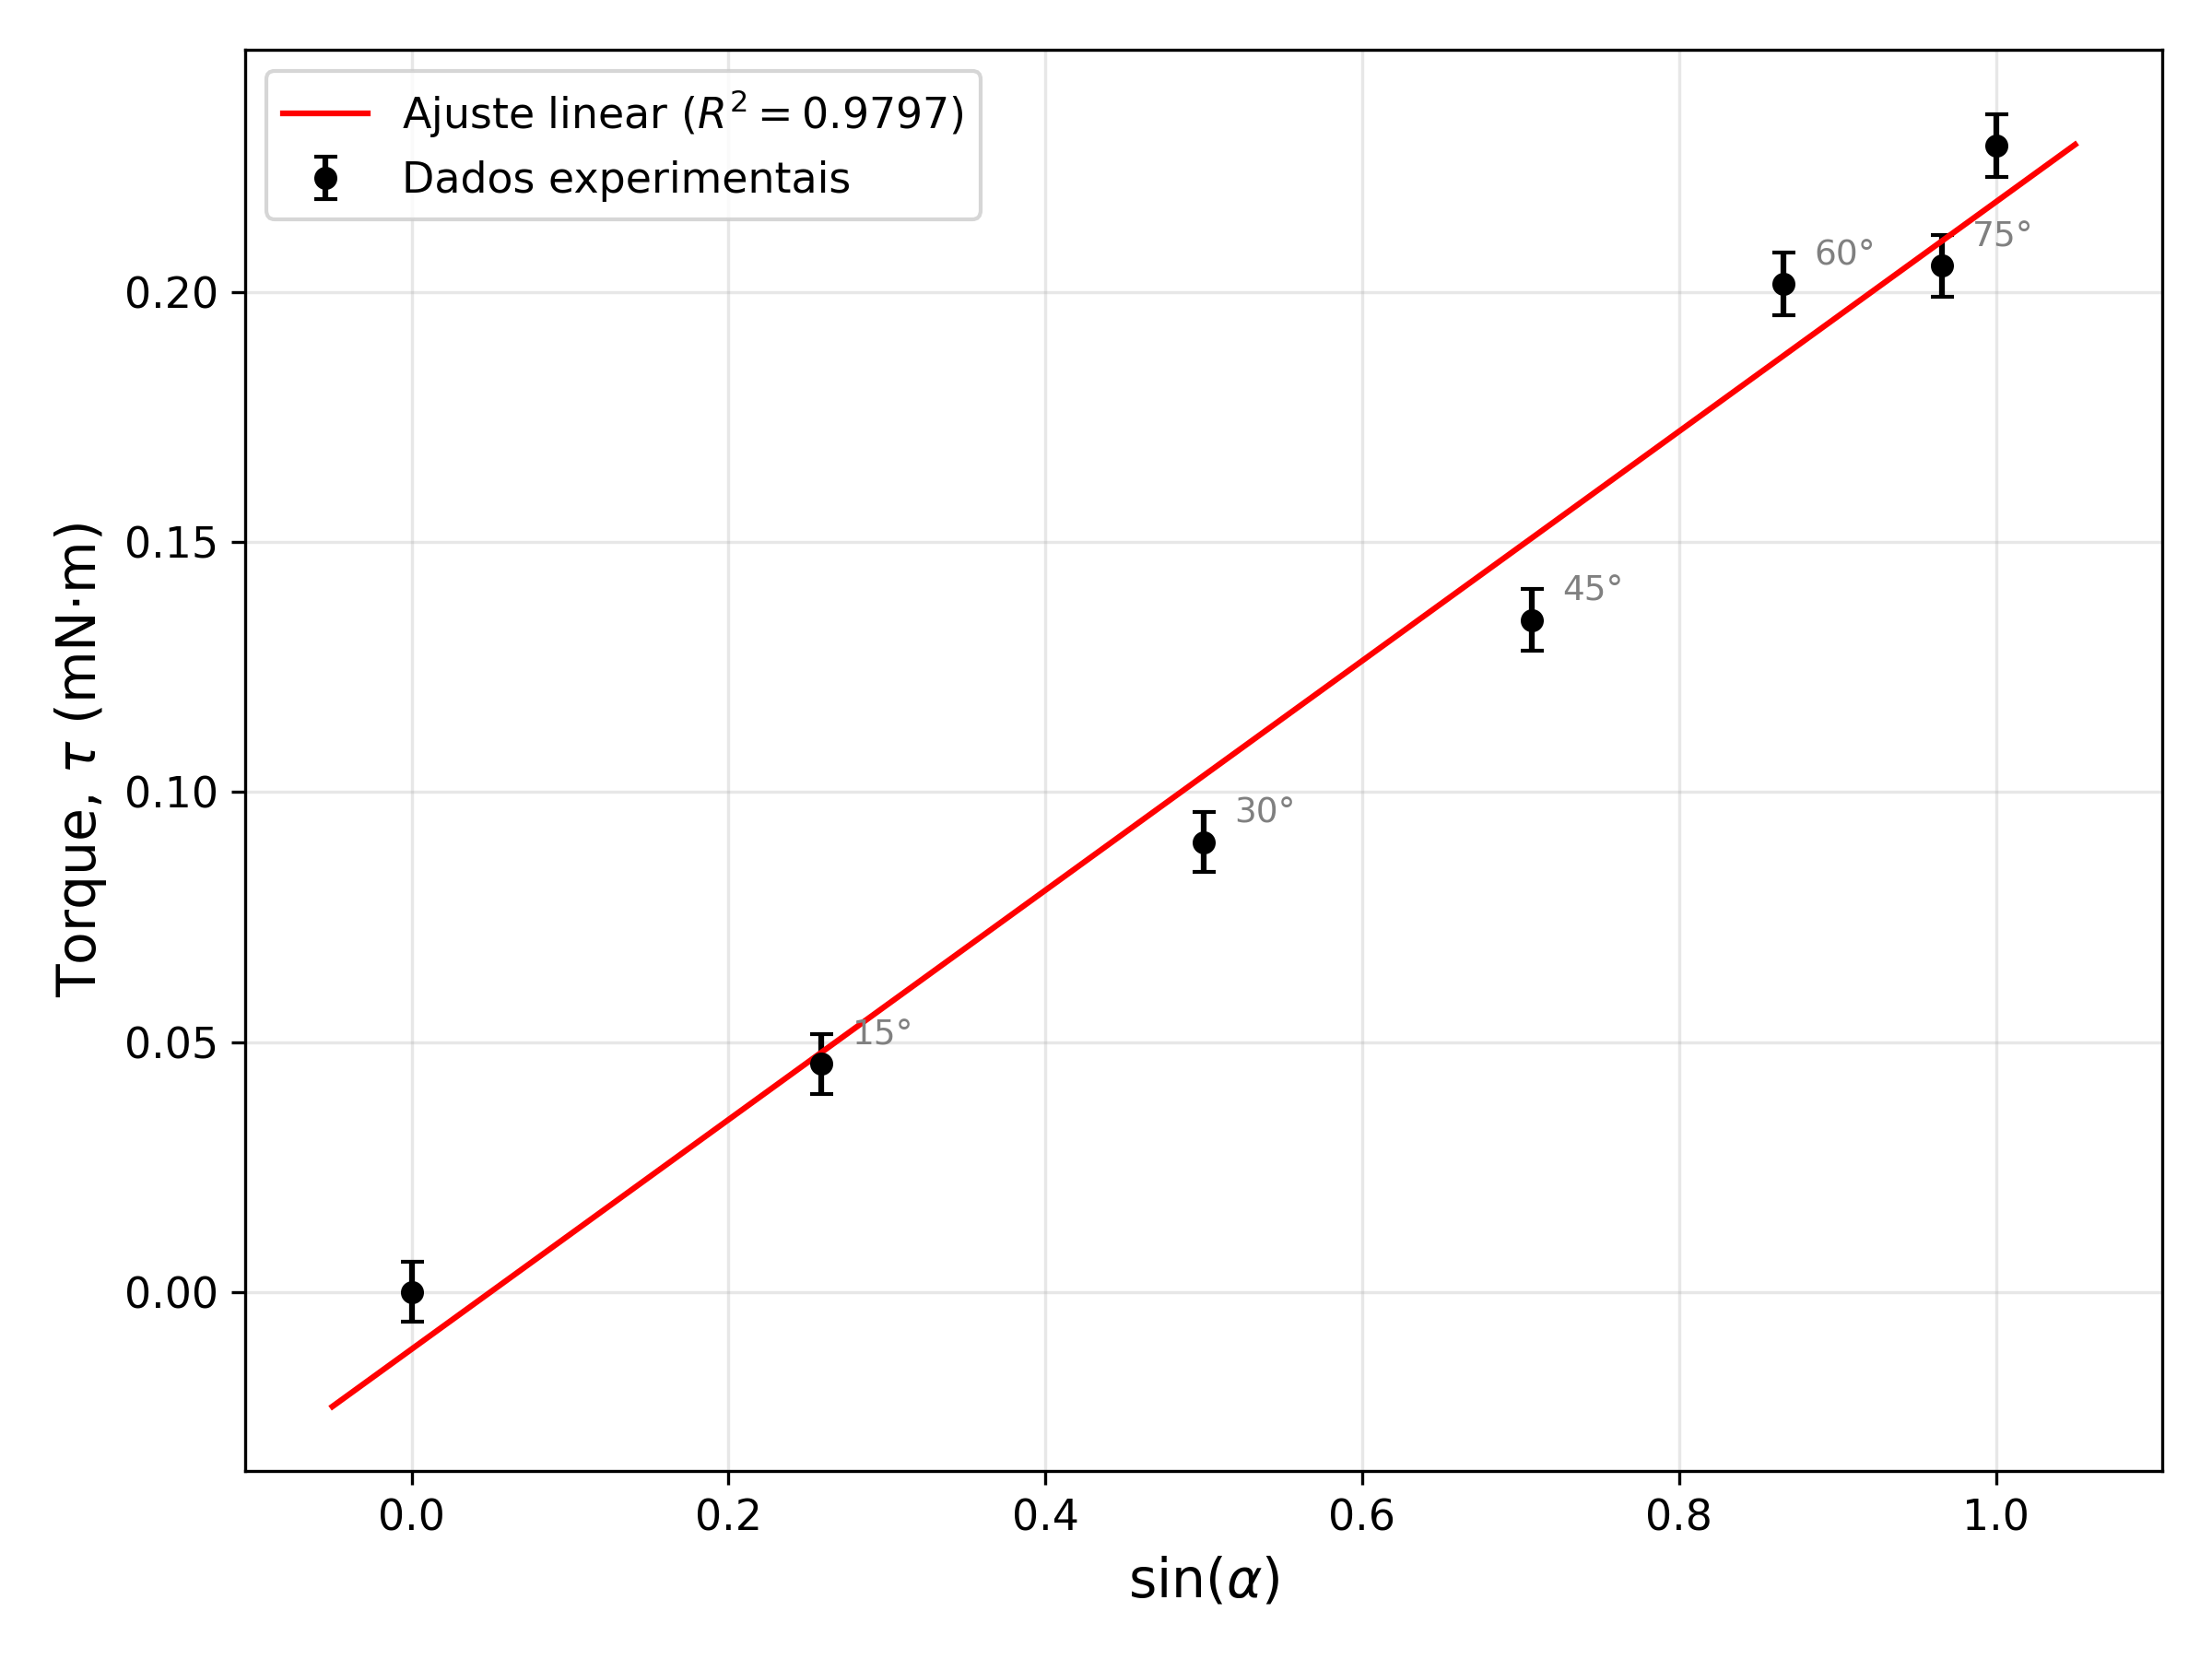
\includegraphics[width=\columnwidth]{tarefa3_tau_vs_sinalpha.png}
  \caption{Tarefa~3: $\tau$ em função de $\sin\alpha$.}\label{fig:t3}
\end{figure}


%% -------------------------------------------------------------------
\subsection{Tarefa 4: $\tau$ \emph{vs.} $d^2$}
%% -------------------------------------------------------------------

A eq.~\eqref{eq:geral} prevê $\tau\propto d^2$. A variável de ajuste é
$x=d^2$ (em \si{\milli\metre\squared}).

\begin{table}[H]
\caption{Tarefa~4: torque em função do diâmetro. Condições fixas: $n=1$,
$I'=\SI{3,032}{\ampere}$, $I=\SI{3,015}{\ampere}$,
$\alpha=\ang{90}$.}\label{tab:t4}
\begin{ruledtabular}
\begin{tabular}{ccccc}
$d$ (mm) & $d^2$ (mm$^2$) & $\sigma_{d^2}$ & $F$ (mN) & $\tau$ (mN$\cdot$m)\\
\hline
59,25  & 3\,510,6  & 5,9 & 0,10 & 0,012 \\
84,20  & 7\,089,6  & 8,4 & 0,20 & 0,024 \\
119,70 & 14\,328,1 & 12,0 & 0,58 & 0,070 \\
\end{tabular}
\end{ruledtabular}
\end{table}

O ajuste linear $\tau = a\,d^2 + b$ fornece
\begin{align}
  a &= \SI{5,5(7)e-6}{\milli\newton\cdot\metre\per\milli\metre\squared}\,,\nonumber\\
  b &= \SI{-0,010(7)}{\milli\newton\cdot\metre}\,,\nonumber\\
  \chi^2_{\text{red}} &= 0{,}89\,,\quad R^2 = 0{,}983\,.\label{eq:fit4}
\end{align}

A verificação pelo gráfico log-log ($\log\tau$ \emph{vs.} $\log d$), mostrada
na Fig.~\ref{fig:t4log}, fornece expoente $\beta=2{,}5\pm0{,}6$, compatível
com o valor teórico~2 dentro de~$1\sigma$ dado o número reduzido de pontos.

\begin{figure}[H]
  \centering
  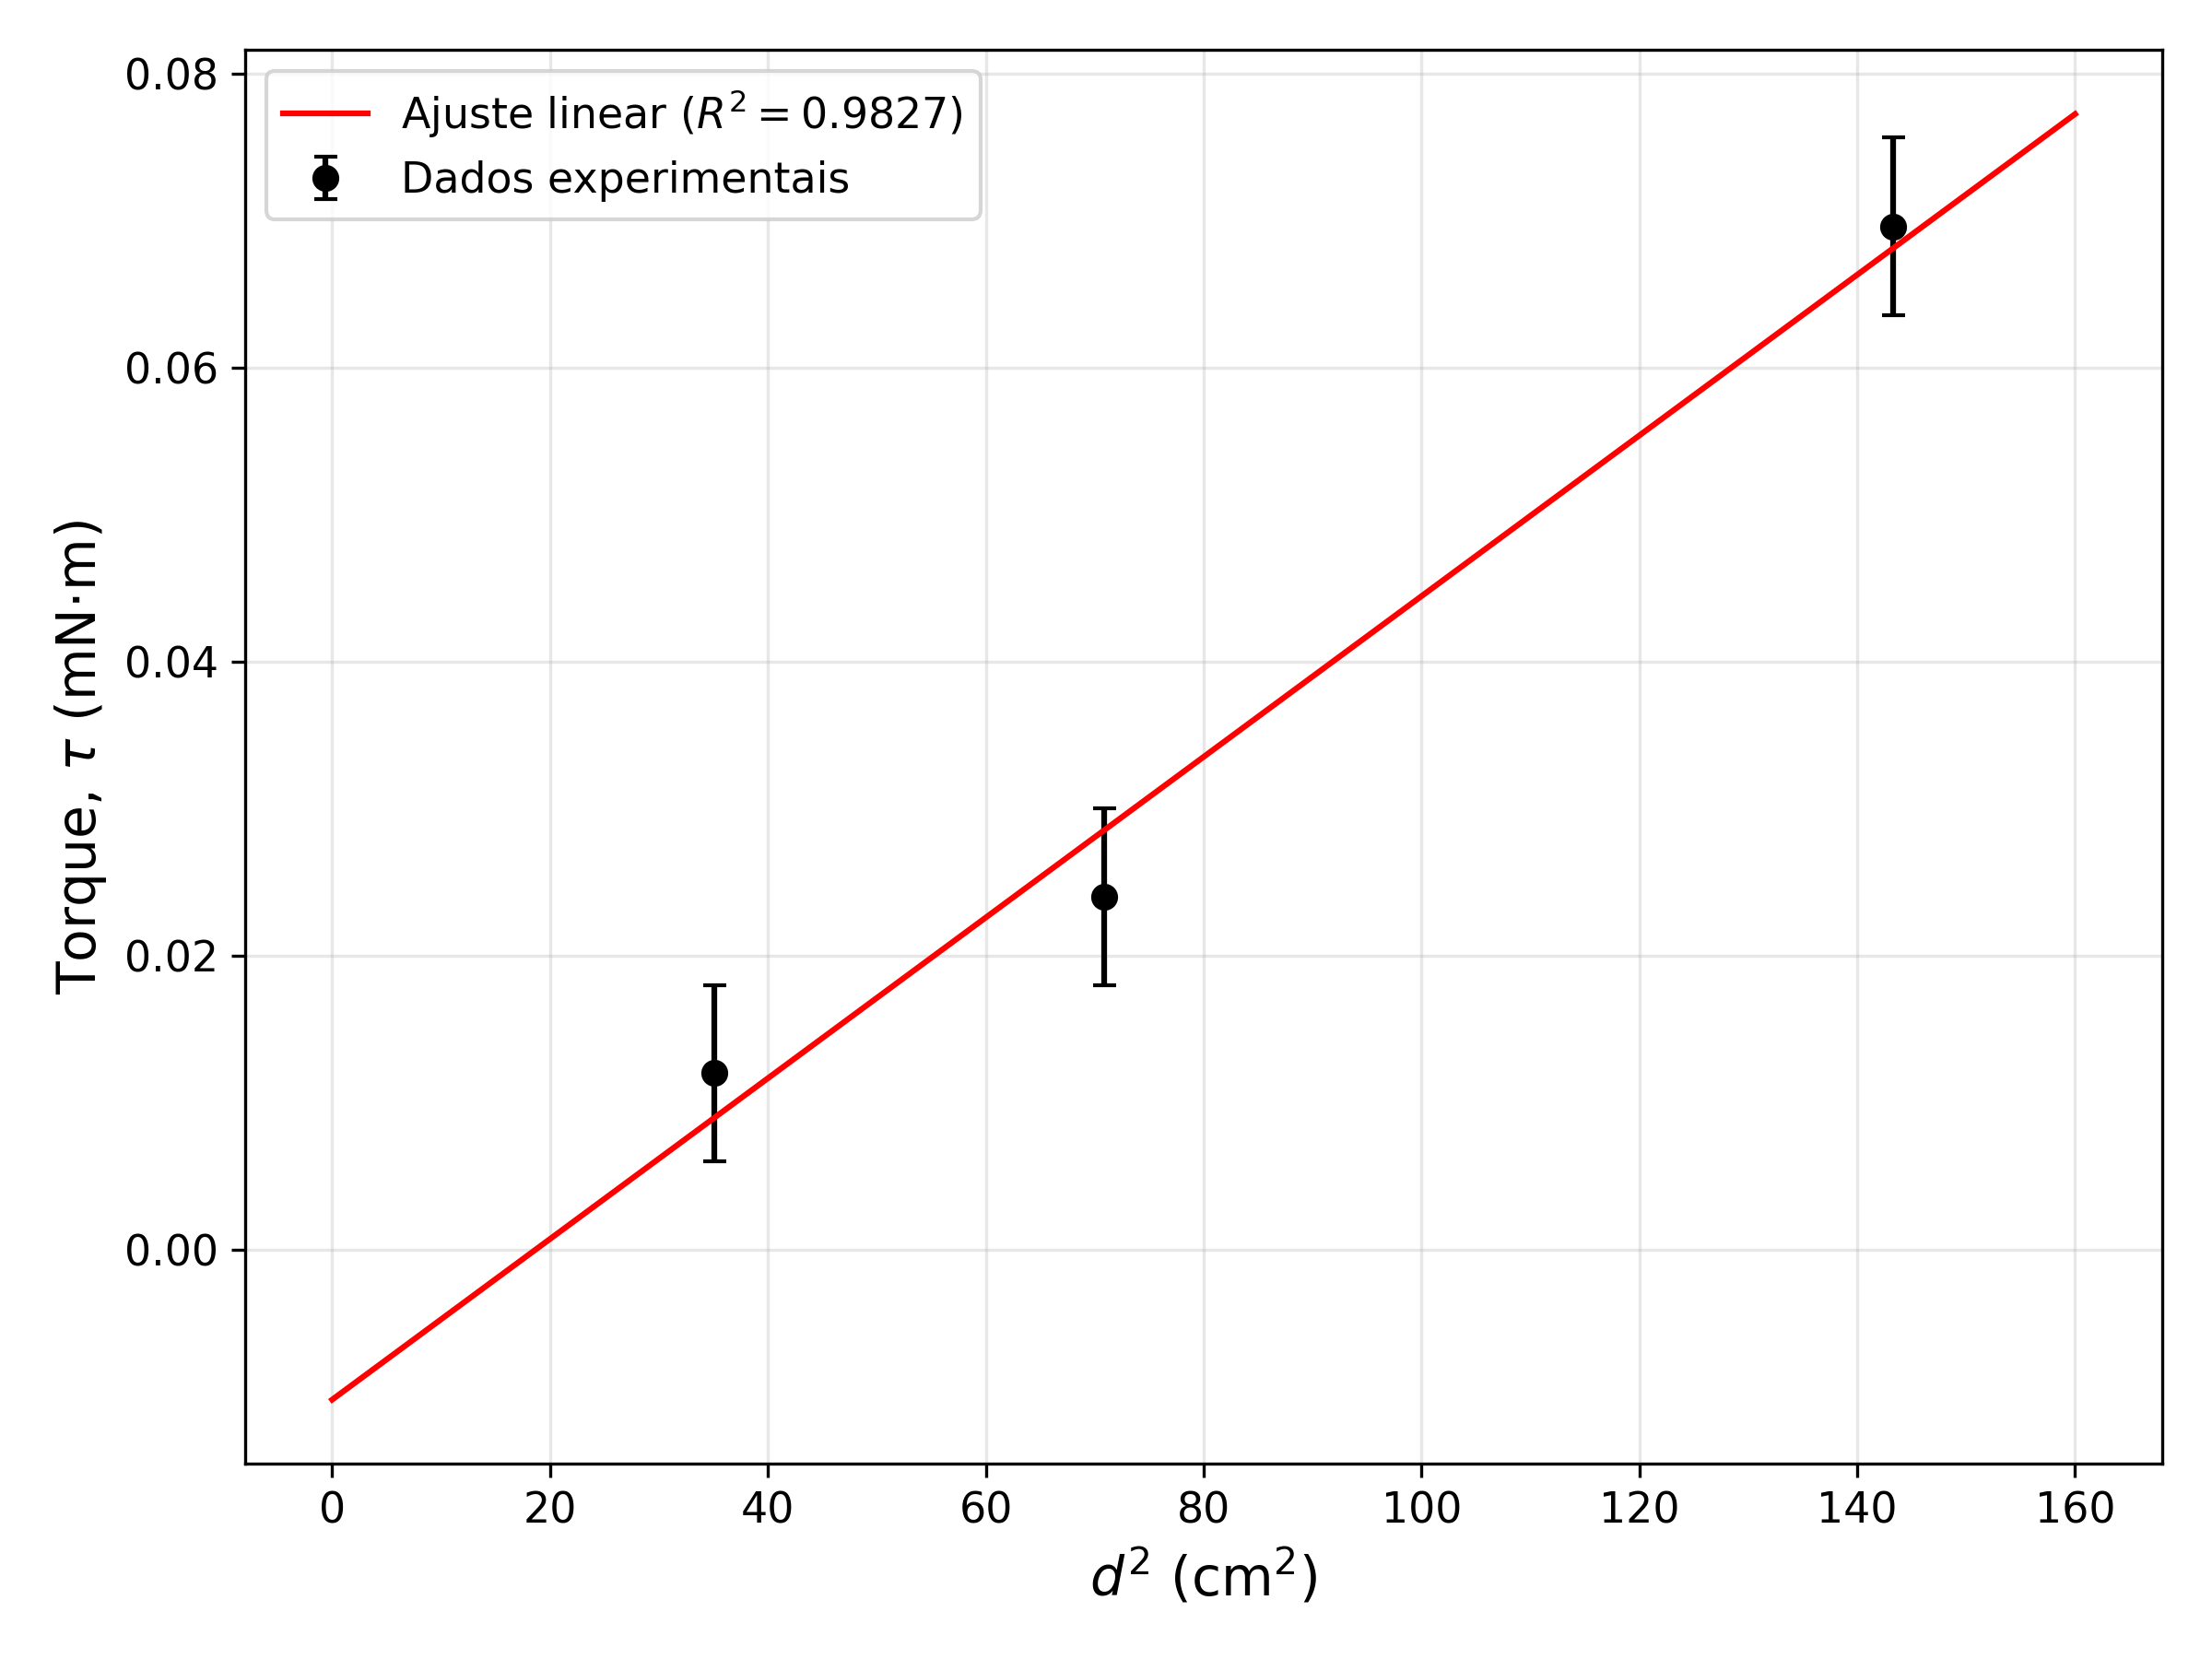
\includegraphics[width=\columnwidth]{tarefa4_tau_vs_d2.png}
  \caption{Tarefa~4: $\tau$ em função de $d^2$. Pontos: dados experimentais.
  Reta: ajuste MMQ ponderado.}\label{fig:t4}
\end{figure}

\begin{figure}[H]
  \centering
  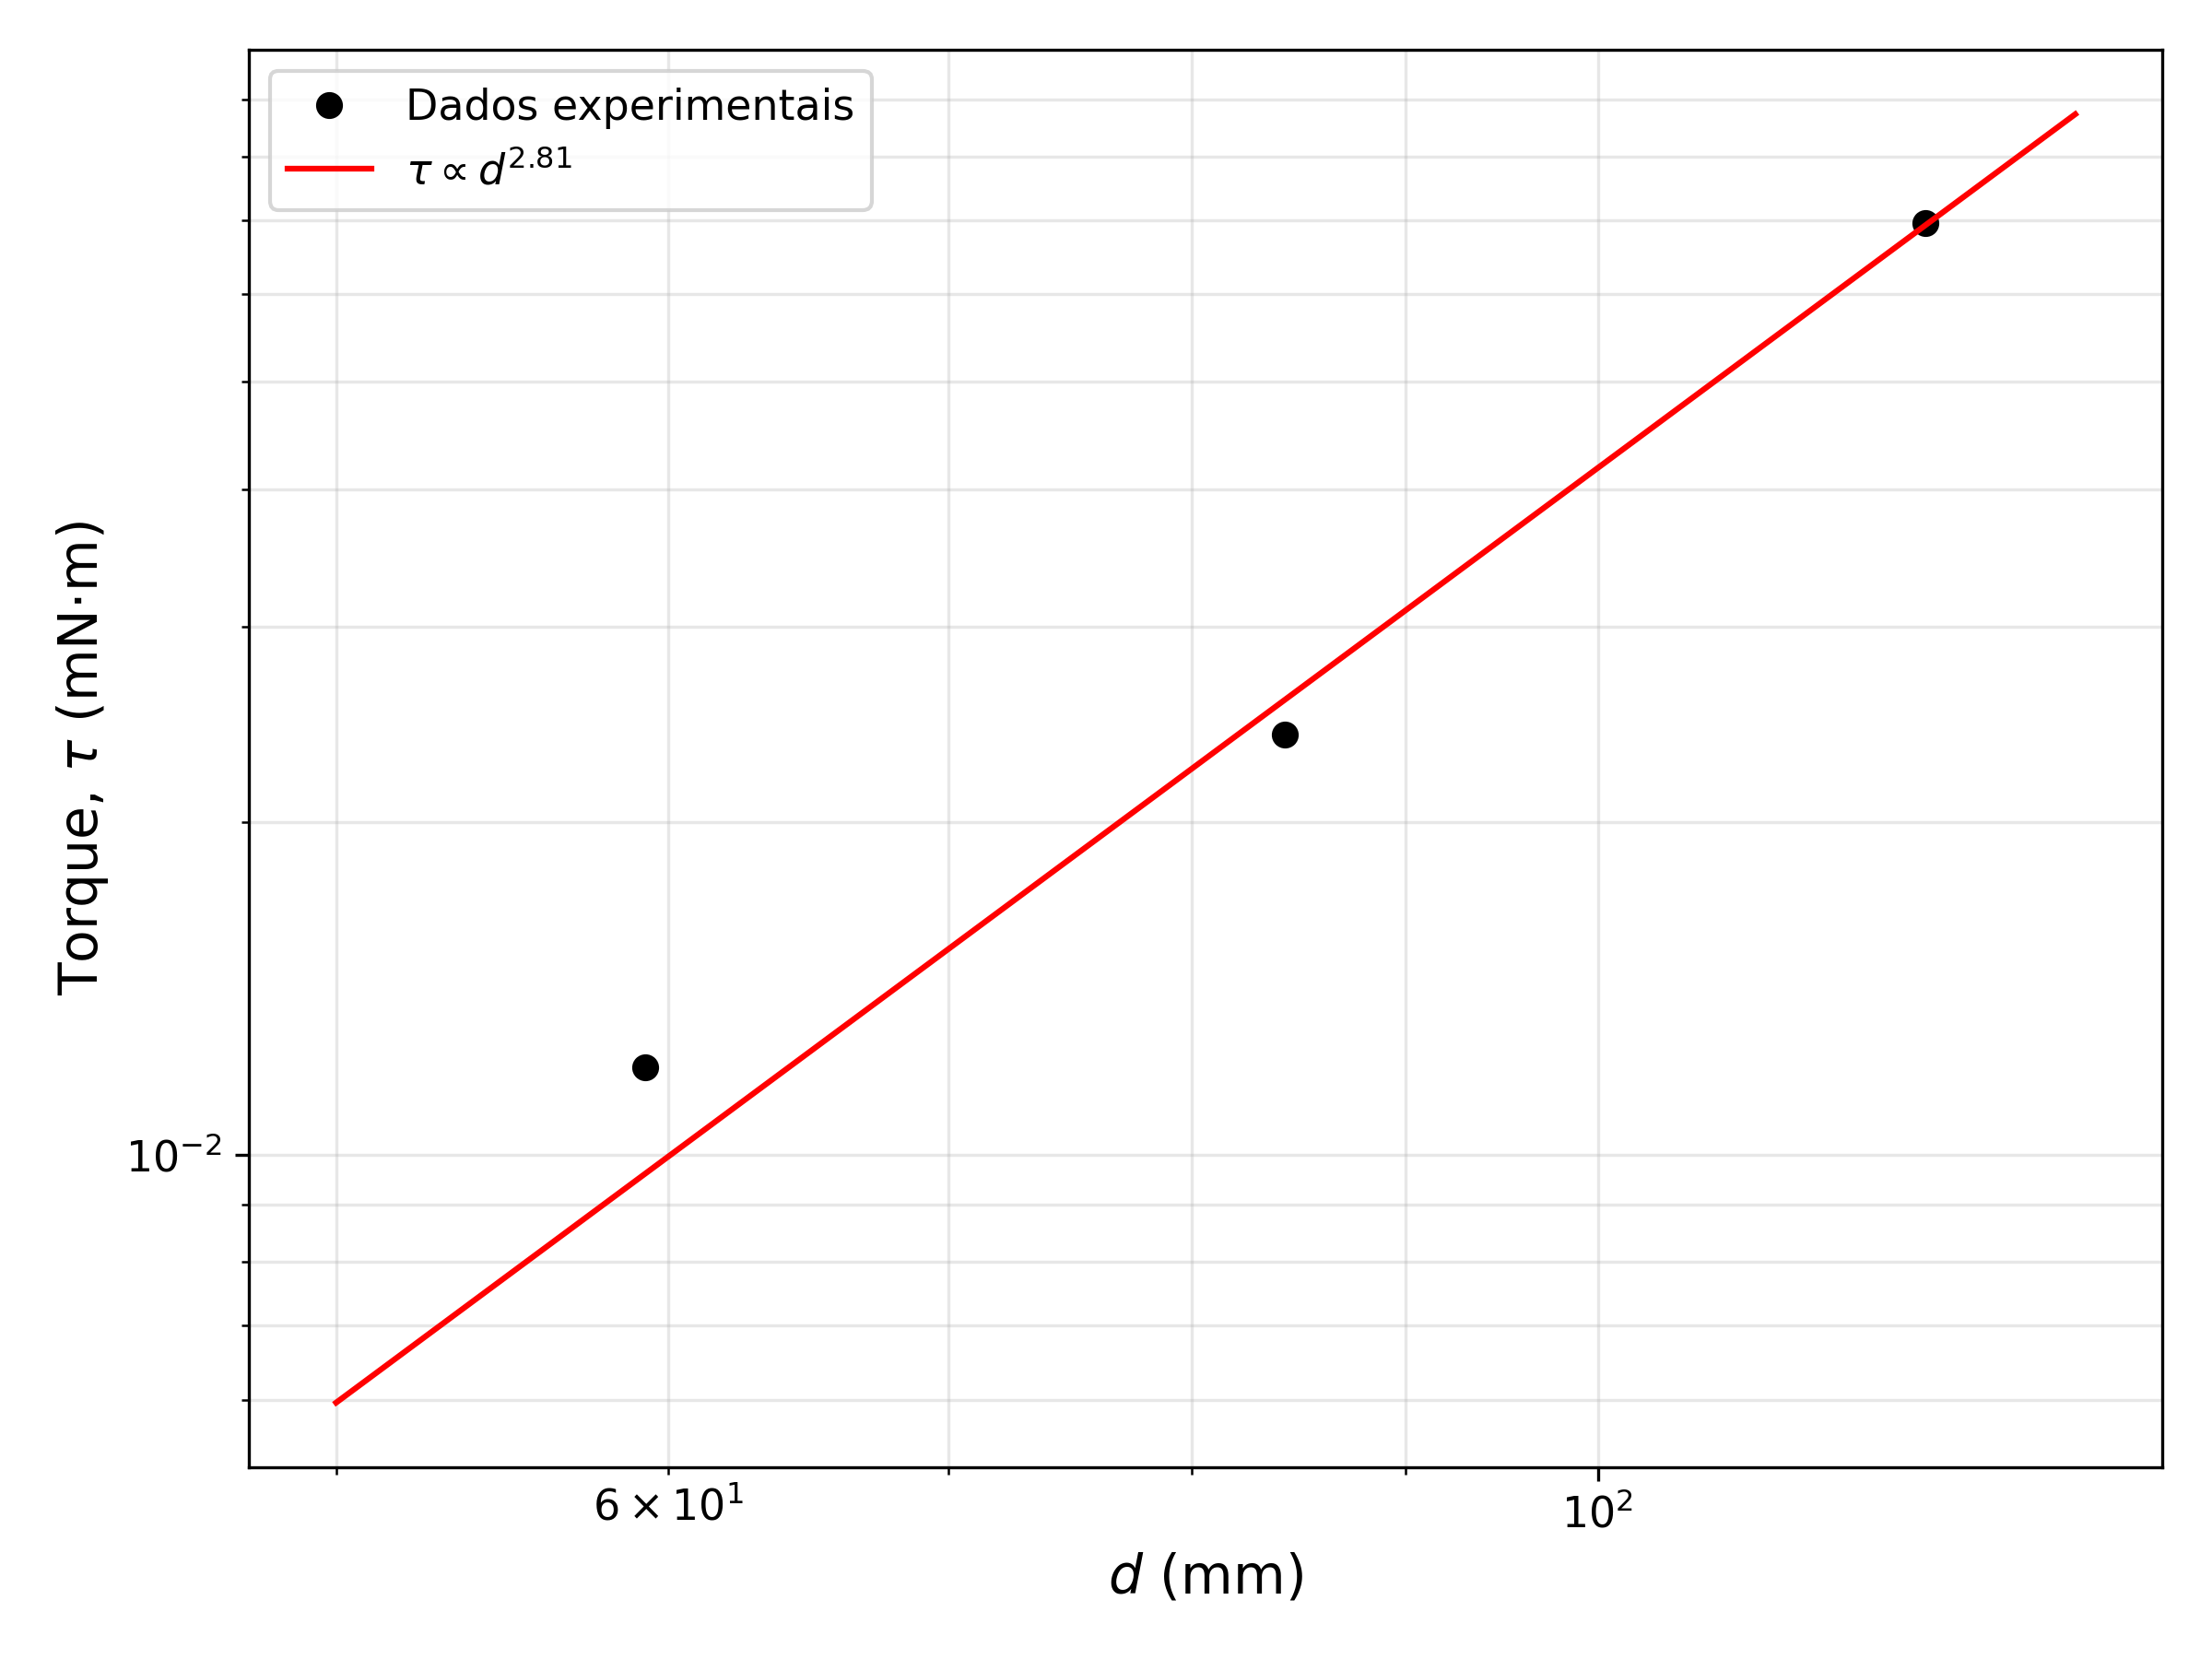
\includegraphics[width=\columnwidth]{tarefa4_loglog.png}
  \caption{Verificação log-log da dependência $\tau\propto d^\beta$.
  Expoente obtido: $\beta=2{,}5\pm0{,}6$.}\label{fig:t4log}
\end{figure}


%% -------------------------------------------------------------------
\subsection{Tarefa 5: $\tau$ \emph{vs.} $I$}
%% -------------------------------------------------------------------

Os dados são apresentados na Tabela~\ref{tab:t5}.

\begin{table}[H]
\caption{Tarefa~5: torque em função da corrente na espira. Condições fixas:
$n=3$, $d=\SI{118,20}{\milli\metre}$, $I'=\SI{3,035}{\ampere}$,
$\alpha=\ang{90}$.}\label{tab:t5}
\begin{ruledtabular}
\begin{tabular}{cccc}
$I$ (A) & $\sigma_I$ (A) & $F$ (mN) & $\tau$ (mN$\cdot$m)\\
\hline
0,309 & 0,012 & 0,21 & 0,025 \\
0,606 & 0,015 & 0,40 & 0,048 \\
0,905 & 0,017 & 0,61 & 0,073 \\
1,207 & 0,020 & 0,74 & 0,089 \\
1,505 & 0,022 & 0,90 & 0,108 \\
1,807 & 0,024 & 1,12 & 0,134 \\
2,105 & 0,027 & 1,30 & 0,156 \\
2,420 & 0,029 & 1,48 & 0,178 \\
2,709 & 0,032 & 1,63 & 0,196 \\
3,008 & 0,034 & 1,82 & 0,218 \\
\end{tabular}
\end{ruledtabular}
\end{table}

O ajuste linear $\tau = a\,I + b$ fornece
\begin{align}
  a &= \SI{0,0710(9)}{\milli\newton\cdot\metre\per\ampere}\,,\nonumber\\
  b &= \SI{0,005(2)}{\milli\newton\cdot\metre}\,,\nonumber\\
  \chi^2_{\text{red}} &= 0{,}14\,,\quad R^2 = 0{,}9988\,.\label{eq:fit5}
\end{align}

\begin{figure}[H]
  \centering
  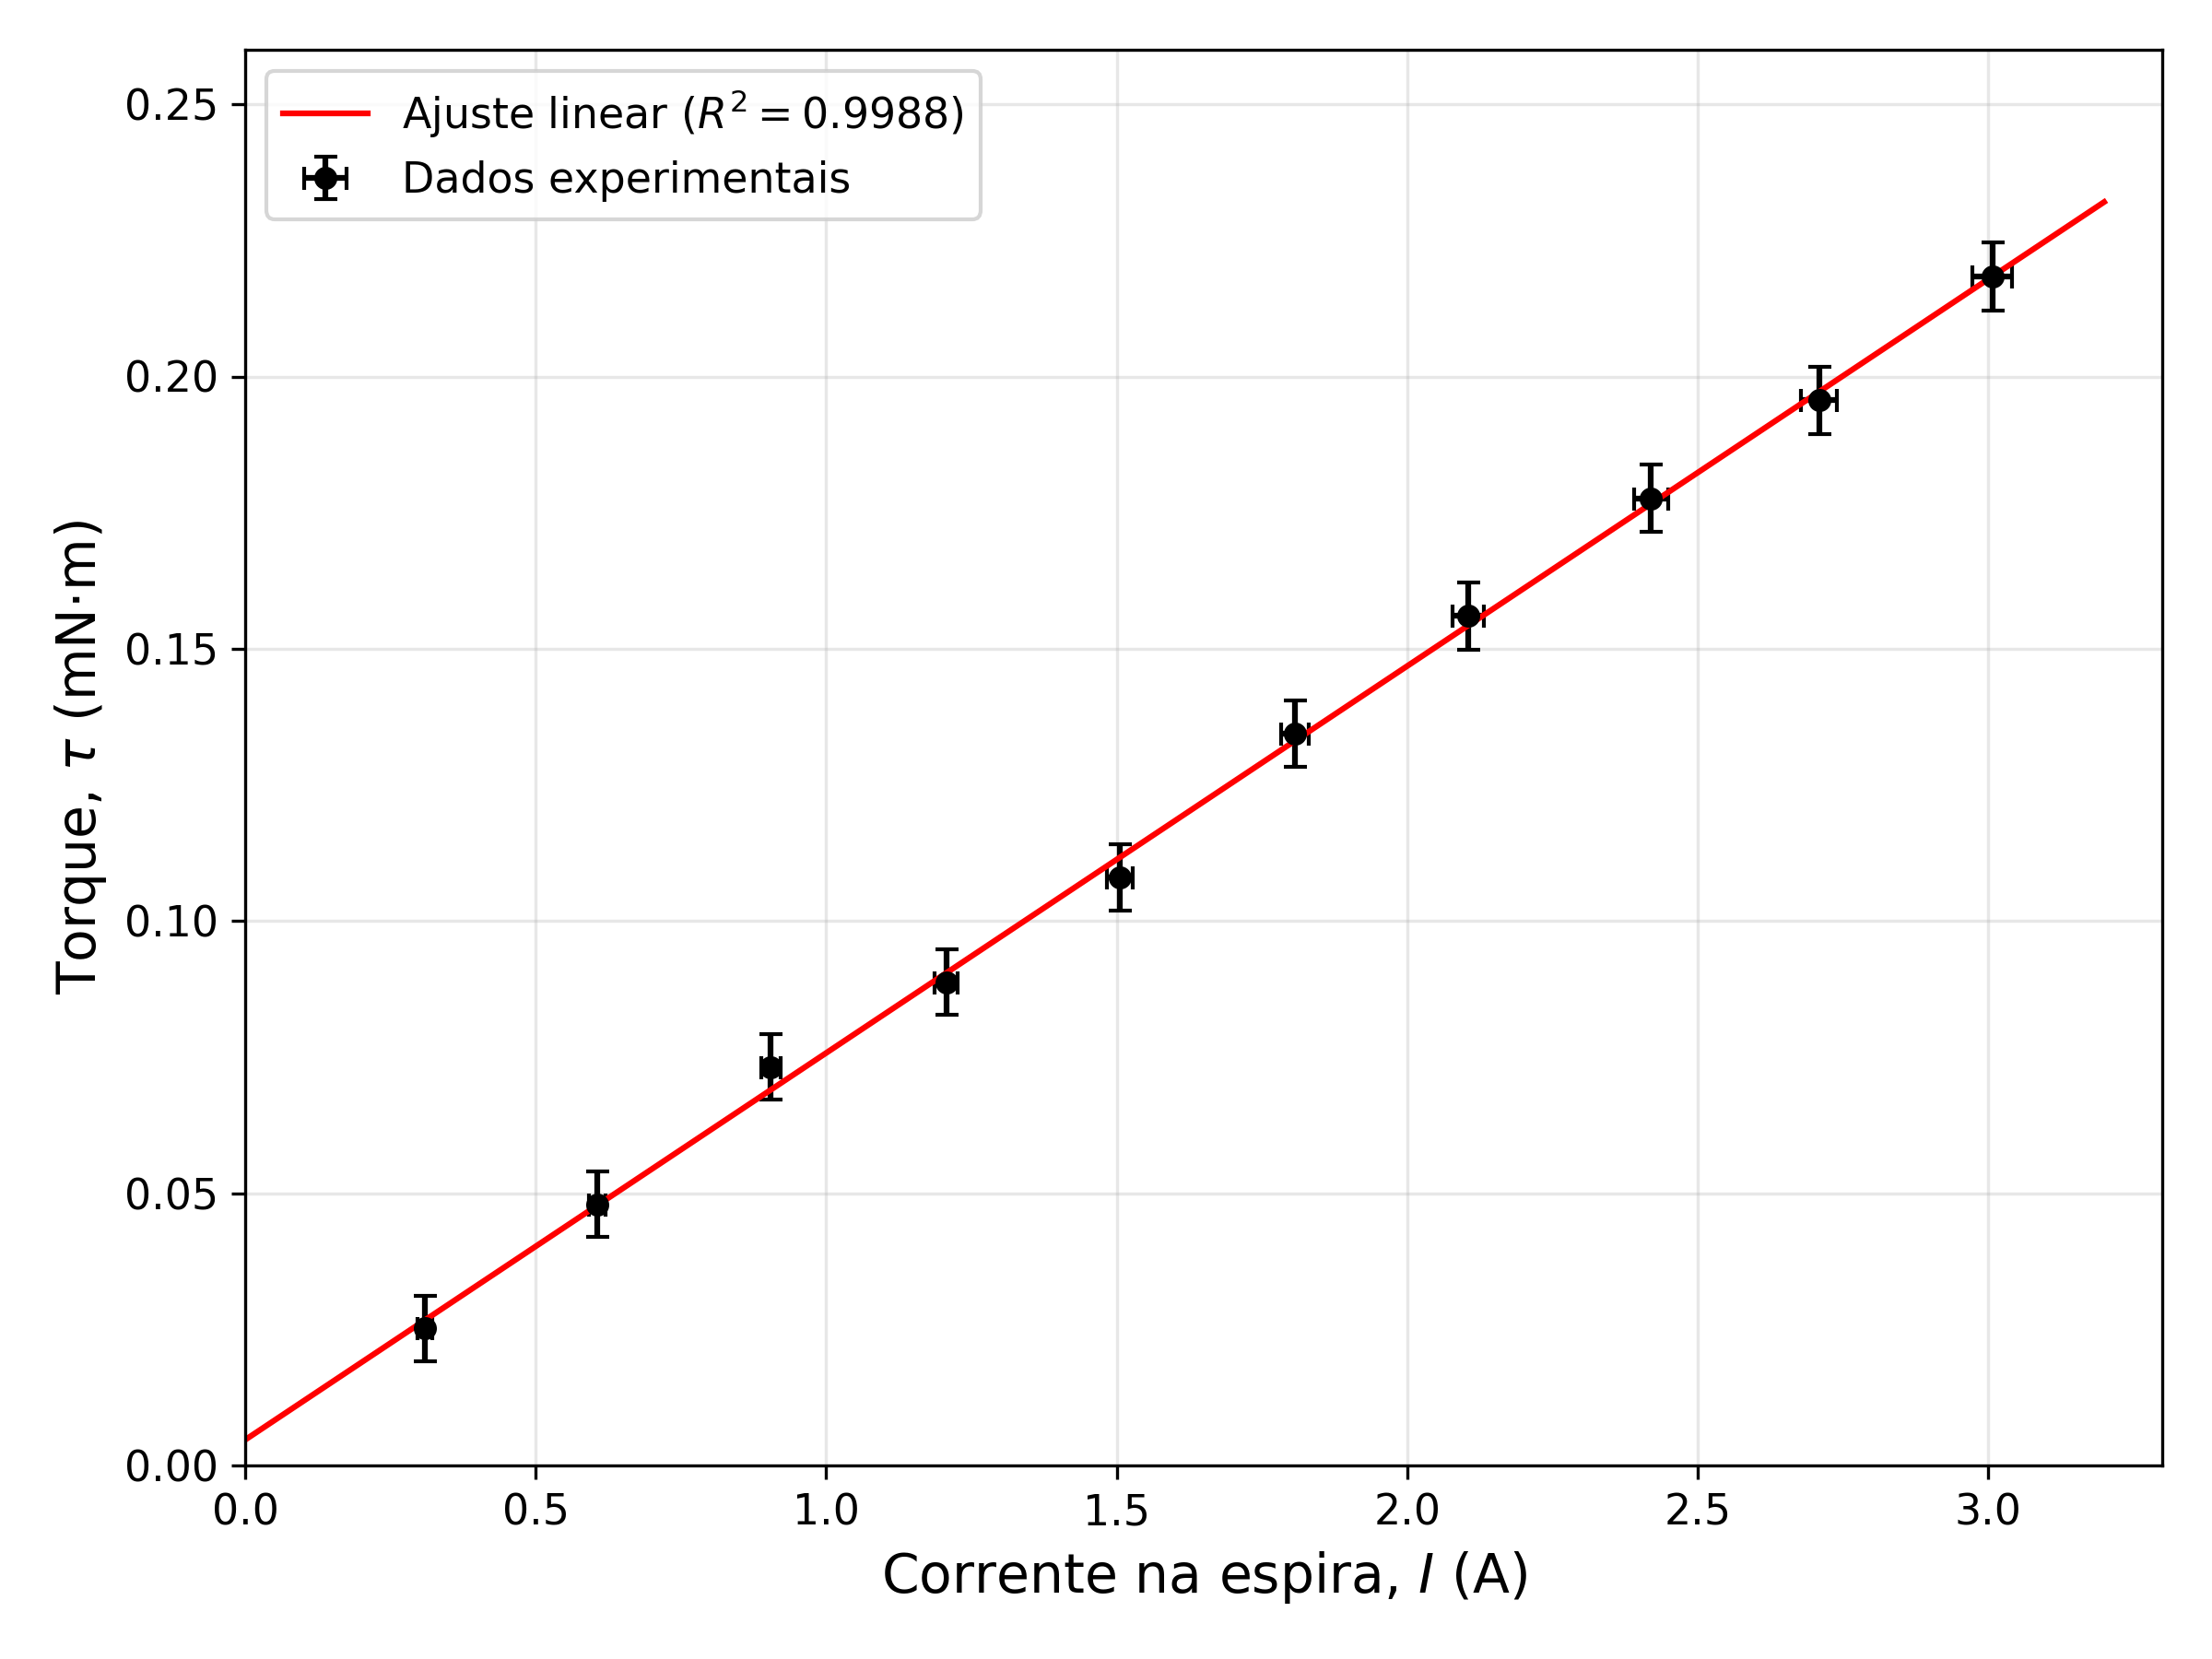
\includegraphics[width=\columnwidth]{tarefa5_tau_vs_I.png}
  \caption{Tarefa~5: $\tau$ em função da corrente na espira~$I$.}\label{fig:t5}
\end{figure}


%% -------------------------------------------------------------------
\subsection{Resumo dos ajustes}
%% -------------------------------------------------------------------

A Tabela~\ref{tab:resumo} reúne os resultados de todos os ajustes.

\begin{table}[H]
\caption{Resumo dos parâmetros de ajuste para as cinco tarefas.}\label{tab:resumo}
\begin{ruledtabular}
\begin{tabular}{ccccc}
Tarefa & Dependência & $\chi^2_\text{red}$ & $R^2$ & $N$ pontos\\
\hline
1 & $\tau$ vs.\ $I'$         & 0,15 & 0,999 & 10 \\
2 & $\tau$ vs.\ $n$          & 7,8  & 0,975 & 3  \\
3 & $\tau$ vs.\ $\sin\alpha$ & 2,9  & 0,979 & 7  \\
4 & $\tau$ vs.\ $d^2$        & 0,89 & 0,983 & 3  \\
5 & $\tau$ vs.\ $I$          & 0,14 & 0,999 & 10 \\
\end{tabular}
\end{ruledtabular}
\end{table}


%% -------------------------------------------------------------------
\subsection{Extração de grandezas físicas}
%% -------------------------------------------------------------------

A partir do coeficiente angular da Tarefa~1, onde $\tau = a\,I'$, e usando
$a = c_\text{exp}\,n\,I\,(\pi d^2/4)$, pode-se extrair a constante
geométrica das bobinas:
\begin{equation}\label{eq:cexp}
  c_\text{exp} = \frac{a}{n\,I\,\pi d^2/4}\,.
\end{equation}
A propagação de incertezas é
\begin{equation}
  \frac{\sigma_c}{c_\text{exp}} = \sqrt{
    \left(\frac{\sigma_a}{a}\right)^2
    + \left(\frac{\sigma_I}{I}\right)^2
    + \left(\frac{2\sigma_d}{d}\right)^2}\,,
\end{equation}
resultando em
\begin{equation}
  c_\text{exp} = \SI{7,31(12)e-4}{\tesla\per\ampere}\,.
\end{equation}

O valor teórico calculado com parâmetros nominais ($n_H=154$,
$R_H=\SI{200}{\milli\metre}$) é $c_\text{teo}=\SI{6,92e-4}{\tesla\per\ampere}$,
isto é, $c_\text{exp}/c_\text{teo}\approx 1{,}06$. A discrepância
$|c_\text{exp}-c_\text{teo}|/\sigma_c\approx 3{,}2$ indica compatibilidade
marginal, discutida na Seção~\ref{sec:discussao}.

O campo magnético para $I'=\SI{3}{\ampere}$ resulta em
$B_\text{exp}=c_\text{exp}\times 3 = \SI{2,19(4)}{\milli\tesla}$, contra
$B_\text{teo}=\SI{2,08}{\milli\tesla}$.

O momento magnético da espira ($n=3$, $I=\SI{3,004}{\ampere}$,
$d=\SI{118,20}{\milli\metre}$) vale
\begin{equation}
  m = n\,I\,A = \SI{98,9(1,1)}{\milli\ampere\cdot\metre\squared}\,.
\end{equation}


%% ====================================================================
\section{Discussão e Conclusão}\label{sec:discussao}
%% ====================================================================

\subsection{Verificação das relações de proporcionalidade}

Todas as cinco dependências previstas pela eq.~\eqref{eq:geral} foram
verificadas com coeficientes $R^2>0{,}97$. Em particular, as Tarefas~1 e~5
apresentam $R^2>0{,}998$ e resíduos aleatórios, indicando excelente
concordância com o modelo linear.

A Tarefa~3 ($\tau$ vs.\ $\sin\alpha$) apresenta $\chi^2_{\text{red}}=2{,}9$,
moderadamente acima de~1. Isso pode ser atribuído a incertezas angulares
subestimadas e ao par de pontos $\alpha=\ang{60}$--$\ang{75}$, cujos valores
de $F$ são praticamente indistinguíveis (\SI{1,68}{\milli\newton} e
\SI{1,71}{\milli\newton}), sugerindo dificuldade experimental na leitura do
dinamômetro para torques próximos ao valor máximo.

A Tarefa~2, com apenas 3~pontos, possui $\chi^2_{\text{red}}=7{,}8$ (1~grau de
liberdade), insuficiente para avaliação estatística rigorosa. A tendência
linear é, no entanto, claramente visível.

\subsection{Qualidade dos ajustes}

Os valores de $\chi^2_{\text{red}}$ das Tarefas 1 e~5 ($\approx 0{,}15$)
indicam que as incertezas experimentais foram ligeiramente superestimadas. Isso
é consistente com a adoção conservadora de
$\sigma_F=\SI{0,05}{\milli\newton}$ (sensibilidade de resposta do
dinamômetro), valor que pode ser maior que a dispersão real das leituras nessas
condições.

Conforme discutido por Vuolo~\cite{Vuolo}, $R^2$ não deve ser usado como única
medida de qualidade de ajuste, pois mede correlação e não verossimilhança
estatística. Os gráficos de resíduos, complementares a $\chi^2_\text{red}$ e
$R^2$, não revelam padrões sistemáticos nas Tarefas 1 e~5.

\subsection{Comparação com valor teórico}

A constante experimental $c_\text{exp}=\SI{7,31(12)e-4}{\tesla\per\ampere}$
está apenas $\sim 6\%$ acima do valor teórico
$c_\text{teo}=\SI{6,92e-4}{\tesla\per\ampere}$, correspondendo a uma
discrepância de $\sim 3\sigma$. Esse nível de acordo é satisfatório para este
tipo de experimento didático. A pequena diferença residual pode ser atribuída a:

(i) Tolerâncias de fabricação nos parâmetros das bobinas de Helmholtz --- o
número real de espiras ou o raio efetivo do enrolamento podem diferir
ligeiramente dos valores nominais ($n_H=154$, $R_H=\SI{200}{\milli\metre}$).

(ii) Imprecisão na determinação do comprimento efetivo do braço de alavanca
$L$ do dinamômetro, cuja incerteza afeta diretamente o valor de $c_\text{exp}$.

(iii) Pequenas não-uniformidades do campo na região ocupada pela espira.

De modo geral, a concordância entre $c_\text{exp}$ e $c_\text{teo}$ confirma a
validade do modelo teórico e a consistência do aparato experimental.

\subsection{Conclusão}

Os resultados confirmam quantitativamente todas as dependências funcionais
previstas pelo modelo $\vec{\tau}=\vec{m}\times\vec{B}$: $\tau\propto I'$,
$\tau\propto n$, $\tau\propto\sin\alpha$, $\tau\propto d^2$ e $\tau\propto I$.
O método dos mínimos quadrados com minimização de $\chi^2$ ponderado mostrou-se
adequado para a análise, e as incertezas instrumentais foram corretamente
propagadas. A constante geométrica experimental das bobinas concorda com o
valor teórico dentro de~$\sim 6\%$, validando tanto o modelo como o
procedimento experimental.


%% ====================================================================
\begin{thebibliography}{9}

\bibitem{Griffiths2017}
D.~J. Griffiths, \textit{Introduction to Electrodynamics}, 4th~ed.\
(Cambridge University Press, Cambridge, 2017).

\bibitem{PHYWE}
PHYWE Systeme GmbH, \textit{Magnetic Moment in the Magnetic Field ---
LEP~4.3.04-00}, Manual de Instruções (Göttingen, Alemanha).

\bibitem{Roteiro}
D.~B. Almeida, Roteiro do Experimento~6 --- Momento Magnético,
Lab.\ de Física Experimental~2 (NHT3028-15), UFABC, 2025.

\bibitem{Vuolo}
J.~H. Vuolo, \textit{Fundamentos da Teoria dos Erros}, 2a~ed.\ (Editora
Edgard Blücher, São Paulo, 1996).

\bibitem{MDM8045A}
Minipa, \textit{Multímetro Digital de Bancada MDM-8045A --- Manual de
Instruções}.

\bibitem{Serway}
R.~A. Serway e J.~W. Jewett Jr., \textit{Princípios de Física}, Vol.~2,
tradução da 5a~ed.\ norte-americana (Cengage Learning, São Paulo, 2015).

\end{thebibliography}
%% ====================================================================

\appendix

\section{Material Suplementar}

Os seguintes arquivos acompanham este relatório:

\begin{itemize}
  \item \texttt{Relatorio\_Jupyter\_Momento\_Magnetico.ipynb} --- Notebook
    Python com análise individual (MMQ ponderado, $\chi^2$, resíduos,
    propagação de incertezas).
  \item \texttt{Dados\_Brutos.ipynb} --- Notebook contendo os dados brutos
    coletados em laboratório.
  \item \texttt{Analise\_e\_Dados\_Brutos\_Momento\_Magnetico.ipynb} ---
    Notebook com a análise aplicada diretamente aos dados brutos.
  \item Repositório GitHub:
    \url{https://github.com/Gsimarelli/Fis.exp2-Momento_Magnetico}
\end{itemize}

A estrutura do código segue o método~I (MMQ com minimização de $\chi^2$): (1)
dados em listas, (2) gráfico de dados brutos com barras de erro, (3)
linearização quando necessária, (4) transferência de incertezas de~$x$
para~$y$, (5) ajuste com \texttt{numpy.polyfit(x,\,y,\,1,\,w=1/$\sigma$,\,cov=True)},
(6) cálculo de $\chi^2_\text{red}$ e $R^2$, (7) gráfico de resíduos, (8)
propagação das incertezas dos parâmetros do ajuste para as grandezas físicas
finais.

\end{document}
